\documentclass[10pt,a4paper,twocolumn,twoside]{article}
\usepackage[utf8]{inputenc}
\usepackage[spanish]{babel}
\usepackage{multicol}
\usepackage{graphicx}
\usepackage{fancyhdr}
\usepackage{times}
\usepackage{titlesec}
\usepackage{multirow}
\usepackage{lettrine}
\usepackage[top=2cm, bottom=1.5cm, left=2cm, right=2cm]{geometry}
\usepackage[figurename=Fig.,tablename=TAULA]{caption}
\usepackage{url}
\usepackage{tabularx}
\usepackage{array}
\usepackage{caption}

\author{\LARGE\sffamily Luis Martínez Zamora}
\title{\Huge{\sffamily Data-Centric AI\@: Mejora de modelos de diagnostico médico mediante pipelines de curación e ingestión automática de vídeo}}
  

\newcommand\blfootnote[1]{%
  \begingroup
  \renewcommand\thefootnote{}\footnote{#1}%
  \addtocounter{footnote}{-1}%
  \endgroup
}

%
%\large\bfseries\sffamily
\titleformat{\section}
{\large\sffamily\scshape\bfseries}
{\textbf{\thesection}}{1em}{}

\begin{document}

\fancyhead[LO]{\scriptsize Luis Martínez Zamora: Data Centric AI\@: Mejora de modelos de diagnostico médico mediante pipelines de curación e ingestión automática de vídeo}
\fancyhead[RO]{\thepage}
\fancyhead[LE]{\thepage}
\fancyhead[RE]{\scriptsize EE/UAB TFG INFORMÀTICA\@: Data-Centric AI}

\fancyfoot[CO,CE]{}

\fancypagestyle{primerapagina}
{
  \fancyhf{}
  \fancyhead[L]{\scriptsize TFG EN ENGINYERIA INFORMÀTICA, ESCOLA D'ENGINYERIA (EE), UNIVERSITAT AUTÒNOMA DE BARCELONA (UAB)}
  \fancyfoot[C]{\scriptsize Marzo~de~2026, Escola d'Enginyeria (UAB)}
}

%\lhead{\thepage}
%\chead{}
%\rhead{\tiny EE/UAB TFG INFORMÀTICA: TÍTOL (ABREUJAT SI ÉS MOLT LLARG)}
%\lhead{ EE/UAB \thepage}
%\lfoot{}
%\cfoot{\tiny{Mes~2026, Escola d'Enginyeria (UAB)}}
%\rfoot{}
\renewcommand{\headrulewidth}{0pt}
\renewcommand{\footrulewidth}{0pt}
\pagestyle{fancy}

%\thispagestyle{myheadings}
\twocolumn[\begin{@twocolumnfalse}

%\vspace*{-1cm}{\scriptsize TFG EN ENGINYERIA INFORMÀTICA, ESCOLA D'ENGINYERIA (EE), UNIVERSITAT AUTÒNOMA DE BARCELONA (UAB)}

\maketitle

\thispagestyle{primerapagina}
%\twocolumn[\begin{@twocolumnfalse}
%\maketitle
%\begin{abstract}
\begin{center}
\parbox{0.915\textwidth}
{\sffamily
\textbf{Resumen--} Este proyecto propone un proceso automatizado basado en el paradigma Data-Centric AI para mejorar la clasificación multiclase de pólipos colorrectales. A través de las técnicas de Visión por Computador clásica se está transformando un conjunto de datos clínicos desequilibrados en homogéneos. El objetivo es demostrar empíricamente que la curación sistemática de los datos de entrenamiento maximiza el rendimiento de un modelo base.
\\
\\
\textbf{Palabras clave-- } Data-Centric AI, Computer Vision, Pytorch, Colonoscopia, Clasificación multiclase \\
\\
%\end{abstract}
%\bigskip
%\begin{abstract}
\bigskip
\\
\textbf{Abstract--} This project proposes an automated pipeline based on the Data-Centric AI paradigm to improve the multiclass classification of colorectal polyps. Using classical Computer Vision techniques, a highly imbalanced clinical dataset is transformed into a homogeneous one. The objective is to empirically demonstrate how systematic data curation maximizes the performance of a lightweight baseline model.
\\
\\
\textbf{Keywords-- } Data-Centric AI, Computer Vision, Pytorch, Colonoscopy, Multiclass Classification.\\
}


{\vrule depth 0pt height 0.5pt width 4cm\hspace{7.5pt}%
\raisebox{-3.5pt}{\fontfamily{pzd}\fontencoding{U}\fontseries{m}\fontshape{n}\fontsize{11}{12}\selectfont\char70}%
\hspace{7.5pt}\vrule depth 0pt height 0.5pt width 4cm\relax}

\end{center}

%\end{abstract}
\end{@twocolumnfalse}]

\section{Introducción y objetivos}

\blfootnote{$\bullet$ E-mail de contacte: lmzamoraa@gmail.com}
\blfootnote{$\bullet$ Menció: Computació}
\blfootnote{$\bullet$ Treball tutoritzat per: Yael Tudela (Ciències de la Computació)}
\blfootnote{$\bullet$ Curs 2025/26}

\lettrine[lines=3]{E}{l} cáncer colorrectal es el tercer cáncer más común a nivel mundial según la Organización Mundial de la Salud (OMS)\cite{who_colorectal_2024}, situándose además entre las principales causas de mortalidad oncológica. Por ello, la prevención y la detección temprana de esta enfermedad resultan fundamentales para reducir su impacto clínico.

En la práctica clínica, la colonoscopia no suele constituir siempre la primera prueba de detección del cáncer colorrectal. Existen distintas estrategias de cribado, entre ellas las pruebas basadas en heces, que son menos invasivas\cite{american_cancer_society_colon}. Sin embargo, cuando el resultado de estas pruebas sugiere la posible presencia de cáncer o de lesiones precursoras, es necesario realizar una colonoscopia para confirmar el hallazgo y continuar el estudio diagnóstico. Por este motivo, aunque no siempre representa la puerta de entrada al proceso asistencial, la colonoscopia ocupa un papel central en el diagnóstico del cáncer colorrectal, ya que permite identificar pólipos y otras lesiones directamente sobre la mucosa e incluso contribuir a la prevención de la enfermedad al detectar lesiones precancerosas.

La colonoscopia\cite{mayoclinic_colonoscopia} es un procedimiento médico cuyo objetivo es examinar el interior del intestino grueso y el recto. Para ello, se introduce por el ano un instrumento denominado colonoscopio, un tubo flexible equipado con una cámara y una fuente de luz en su extremo. Esta técnica permite la visualización directa y en tiempo real de la mucosa intestinal, lo que la convierte en una herramienta especialmente útil para detectar úlceras, inflamaciones, tumores y, en el contexto de este trabajo, pólipos. La identificación precisa de estas lesiones precancerosas durante la exploración en vídeo es crítica, ya que su detección temprana reduce de forma significativa el riesgo de progresión a cáncer colorrectal.

Actualmente, la evaluación de pólipos durante una colonoscopia se realiza principalmente mediante la observación visual del médico especialista. Sin embargo, esta tarea puede resultar compleja debido a la variabilidad en la apariencia anatómica de las lesiones, las condiciones de iluminación y la presencia de artefactos visuales. En este contexto, el uso de técnicas de inteligencia artificial para asistir en el análisis automatizado de colonoscopias ha despertado un interés creciente.

Respecto a las posibles lesiones, los pólipos no son un grupo homogéneo, sino que presentan diversas histologías que exigen protocolos de actuación y tratamientos distintos. Gran parte de los sistemas automatizados existentes se han limitado a desarrollar clasificadores binarios que discriminan únicamente entre lesiones neoplásicas (como los adenomas precancerosos) y no neoplásicas (pólipos benignos). No obstante, la realidad clínica es más compleja que una simple distinción binaria entre lesiones neoplásicas y no neoplásicas. En el contexto de este trabajo, se ha optado por una clasificación en cuatro clases —adenomas, adenomas serrados sésiles, pólipos hiperplásicos y adenocarcinomas— porque cada una de ellas representa una situación clínica diferente y aporta un nivel de detalle diagnóstico relevante. Los pólipos hiperplásicos suelen asociarse a un potencial maligno muy bajo, mientras que los adenomas constituyen precursores del cáncer colorrectal. Por su parte, las lesiones serradas sésiles también pueden actuar como precursoras, pero a través de una vía biológica distinta y con una apariencia más sutil, lo que incrementa su dificultad de detección. Finalmente, el adenocarcinoma representa una lesión maligna ya establecida, con implicaciones clínicas claramente diferenciadas respecto al resto de categorías consideradas en este trabajo, que corresponden a lesiones benignas o premalignas. Por ello, limitar el problema a dos clases reduciría la complejidad real del escenario clínico y ocultaría diferencias relevantes para el diagnóstico y la toma de decisiones médicas.\cite{rex2012,nih_colon_treatment}

Computacionalmente, esta transición de una clasificación binaria a una multiclase introduce un problema crítico: cada variante presenta diferencias sutiles y una frecuencia de aparición muy dispar en la población general. Esto genera un severo desbalanceo natural de las muestras, donde la escasez de imágenes para las tipologías menos comunes provoca que los clasificadores estándar pierdan eficacia.

Los conjuntos de datos clínicos presentan dificultades estructurales que los diferencian de otros problemas de visión artificial más controlados. En primer lugar, suelen estar marcados por un fuerte desbalanceo de clases, ya que las lesiones más frecuentes concentran gran parte de las muestras mientras que las patologías menos comunes aparecen escasamente representadas. Esto, sumado a la variabilidad de cada lesión entre pacientes y la necesidad de anotaciones expertas, limita la disponibilidad de datos. En consecuencia, el rendimiento de los modelos no depende únicamente de la arquitectura utilizada, sino también de la calidad y representatividad del conjunto de entrenamiento.\cite{salmi2024imbalanced}

Tradicionalmente, gran parte de la investigación en inteligencia artificial médica ha abordado este tipo de problemas desde un enfoque \textit{model-centric}. Bajo este paradigma, la mejora del sistema se persigue principalmente mediante modificaciones en la arquitectura, ajustes de hiperparámetros, estrategias de entrenamiento más complejas o combinaciones de múltiples modelos. Aunque este enfoque puede producir mejoras en entornos experimentales, en el ámbito clínico presenta limitaciones como el incremento del coste computacional, lo que dificulta el despliegue en tiempo real y, sobre todo, no corrige de forma directa los defectos estructurales del conjunto de datos. Cuando el origen del problema se encuentra en el ruido, la redundancia o el desbalanceo de las muestras, aumentar la complejidad del modelo no siempre se traduce en una mejora robusta del sistema.\cite{zha2025datacentric}

Frente a esta perspectiva, el paradigma \textit{Data-Centric AI} propone trasladar el foco principal de la ingeniería desde el modelo hacia los datos. Este enfoque se basa en diseñar y refinar sistemáticamente los datos, asumiendo una arquitectura relativamente estable y concentrando el esfuerzo en mejorar la calidad del conjunto de entrenamiento.\cite{ng_datacentric} Esta visión ha sido posteriormente consolidada por la comunidad investigadora, que la describe como una transición desde la mejora del modelo hacia el tratamiento de problemas como la recolección de datos, el etiquetado, el preprocesado y la evaluación de calidad del dato.\cite{zha2025datacentric}

Este trabajo se sitúa explícitamente dentro de este último paradigma. En lugar de plantear sucesivas iteraciones sobre arquitecturas cada vez más complejas, se fija un modelo \textit{baseline} ligero y se concentra la contribución principal en la construcción de un pipeline de software orientado a mejorar los datos de entrenamiento. Dicho pipeline aborda de forma secuencial la ingestión automática de imágenes a partir de vídeo, el filtrado de calidad de imagen, la reducción de redundancia temporal y el reequilibrado de clases. De este modo, la hipótesis central del TFG no es que un modelo más complejo resuelva mejor el problema, sino que una mejora sistemática y reproducible de los datos clínicos puede aumentar de forma significativa la capacidad predictiva de un clasificador estándar.\cite{zha2025datacentric, ng_datacentric}

\subsection{Objetivos}
\subsubsection{Objetivo principal}
Desarrollar un pipeline automatizado de curación e ingestión de datos a partir de vídeo bajo el paradigma Data-Centric AI, evaluando de forma iterativa la evolución del rendimiento de un modelo baseline específico, en este caso será una arquitectura ligera pre-entrenada del tipo EfficientNet\cite{tan2019efficientnet}, fijando los hiperparámetros que se utilizarán a lo largo de todo el proceso. La elección de esta arquitectura ligera busca reducir la carga computacional, permitiendo iteraciones rápidas para evaluar el impacto de las mejoras en los datos.

El propósito es cuantificar la mejora progresiva del clasificador paso a paso mediante métricas de evaluación robustas frente al desbalanceo de clases, específicamente F1-Score macro además de la realizar la matriz de confusión para tener todas las métricas. Con esto se busca demostrar empíricamente que la optimización sistemática de los datos de entrenamiento es un factor determinante para maximizar la capacidad predictiva del sistema, superando al conjunto de datos original estático.
\subsubsection{Objetivos secundarios}
\begin{itemize}
    \item Construir un módulo de software eficiente para la ingestión y procesamiento de vídeos de colonoscopias que permita la extracción inteligente de frames a partir de las marcas temporales (timestamps) etiquetadas por los especialistas. En lugar de una extracción contigua basada en ventanas fijas, el sistema implementará técnicas de Visual Object Tracking (VOT) basadas en el paradigma Tracking-by-Detection, con un modelo de detección YOLO junto al algoritmo ByteTrack\cite{zhang2022bytetrack}, ya que este seguirá el rastro del pólipo en situaciones donde la calidad de la imagen baja drásticamente, permitiendo encontrar imagenes de buena calidad. Esto permitirá buscar en la cercanía temporal del frame original para extraer perspectivas alternativas del mismo pólipo y, simultáneamente, corregir errores de etiquetado manual seleccionando automáticamente el frame de mayor calidad óptica si el original carece de valor diagnóstico. Hay que destacar que esta etapa de extracción será más restrictiva con clases mayoritarias, buscando reducir así el desbalanceo.
    \item Implementar un algoritmo secuencial de descarte mediante técnicas de Visión Artificial clásica para para la limpieza de los datos. El pipelina funcionará eliminando automáticamente frames sin valor diagnóstico en un orden específico para optimizar la carga computacional: descarte por oscuridad, presencia excesiva del lúmen anatómico, falta de textura por colisión contra la mucosa, y finalmente, desenfoque por movimiento de la cámara.
    \item Implementar algoritmos de similitud visual, haciendo uso de técnicas como Perceptual Hashing (pHash) o métricas como Structural Similarity Index Measure (SSIM), para identificar secuencias de frames temporalmente redundantes. Sobre estos grupos, se aplicará una política de selección para extraer los $X$ frames de mayor calidad óptica. Esta selección se automatizará calculando un Quality Score basado en la maximización de la nitidez (mediante la Varianza del Laplaciano) y el área de la lesión detectada, garantizando así la máxima riqueza visual para el entrenamiento y previniendo el overfitting.
    \item Definir y ejecutar un marco de experimentación que registre y compare las métricas del modelo tras la aplicación sucesiva de cada módulo del pipeline, aislando y demostrando el impacto individual de cada técnica.
\end{itemize}

\section{Planificación temporal}
Para asegurar el correcto desarrollo del TFG, se ha establecido un cronograma (Fig.\ref{fig:gantt_tfg}) que divide el trabajo en bloques.

\begin{figure}[htbp]
    \centering
    \includegraphics[width=0.49\textwidth]{timeline.pdf}
    \caption{Diagrama de Gantt del desarrollo del TFG.}
    \label{fig:gantt_tfg}
\end{figure}

\subsection{Seguimiento de la planificación}
Hasta la fecha de entrega de este informe, el desarrollo del TFG ha seguido de forma general la planificación definida en el informe inicial. En concreto, se han completado dentro del periodo previsto las tres primeras fases del proyecto.
Esto permite mantener como siguiente objetivo la fase 4 del proyecto, centrada en la reducción de redundancia temporal mediante técnicas de similitud visual y selección de frames representativos.

\begin{table}[htbp]
\centering
\caption{Seguimiento de la planificación hasta Progrés I}
\label{tab:seguimiento_planificacion}
\scriptsize
\resizebox{\columnwidth}{!}{%
\begin{tabular}{l l l l}
\hline
\textbf{Fase} &  \textbf{Estado actual}  \\
\hline
Fase 1: Baseline  & Completada  \\
Fase 2: Ingestión  & Completada  \\
Fase 3: Limpieza  & Completada \\
Fase 4: Deduplicación  & Pendiente  \\
Fase 5: MLOps y análisis  & Pendiente \\
\hline
\end{tabular}%
}
\end{table}

Por tanto, en el momento actual no se considera necesario modificar la estructura global del plan de trabajo. Aun así, se mantendrá una revisión continua de la carga de trabajo de las fases posteriores para garantizar la finalización del proyecto dentro del calendario previsto.
\section{Metodologia seguida}
\subsection{Fase 1: Entrenamiento del modelo baseline}

\subsubsection{Arquitectura seleccionada}
Como punto de partida del proyecto se define un modelo \textit{baseline} fijo, que actúa como referencia sobre la que se evaluará el impacto de todas las mejoras introducidas posteriormente en los datos. Dado que el objetivo del TFG se enmarca en el paradigma \textit{Data-Centric AI}, no se persigue maximizar el rendimiento mediante iteraciones sucesivas sobre la arquitectura, sino mantener una receta de entrenamiento estable y reproducible para que la evolución de los resultados pueda atribuirse exclusivamente a los cambios aplicados al conjunto de datos.

Para ello se emplea una arquitectura \textit{EfficientNet-B0} preentrenada sobre ImageNet\cite{tan2019efficientnet}, elegida por su buena relación entre capacidad de aprendizaje y coste computacional. Esta elección resulta adecuada para el contexto del proyecto porque permite realizar múltiples iteraciones experimentales con un coste temporal asumible y, al mismo tiempo, suficiente para evaluar el efecto de la curación del dataset sin recurrir a modelos excesivamente complejos.

\subsubsection{Configuración del entrenamiento}
La configuración final del entrenamiento se resume en la Tabla~\ref{tab:baseline_config}, donde se recogen los hiperparámetros relevantes que definen la receta final del \textit{baseline}.

La selección del mejor modelo se realiza atendiendo al valor de F1-score macro en validación, al tratarse de un problema multiclase con fuerte desbalanceo entre clases. De forma complementaria, se analiza la matriz de confusión para estudiar el comportamiento del clasificador en cada categoría histológica.

\subsubsection{Estrategia de fine-tuning}
La optimización sigue un esquema de \textit{fine-tuning} progresivo. Durante las primeras épocas se entrena únicamente la cabeza de clasificación adaptada al problema multiclase, manteniendo congelado el resto de la red. Esta decisión permite estabilizar primero la capa final, que parte de cero y debe aprender correctamente sobre las características visuales hacia las cuatro clases histológicas consideradas.

Una vez finalizado este periodo inicial, se habilita el entrenamiento de la red completa. Esta transición permite aprovechar el conocimiento visual ya presente en los pesos preentrenados, ajustándolo progresivamente al dominio del proyecto, sin modificar desde el inicio todas el conocimiento interno del modelo. En la práctica, esta estrategia resulta más estable que entrenar toda la red desde la primera iteración, ya que reduce el riesgo de deteriorar las características generales base del modelo.

Para acompañar este cambio de fase se definen tasas de aprendizaje diferenciadas. Durante el \textit{warmup}, la cabeza de clasificación se entrena con una tasa de aprendizaje superior, mientras que en la fase de \textit{fine-tuning} completo tanto la cabeza como el \textit{backbone} pasan a optimizarse con valores más bajos, especialmente en el backbone, provocando así una optimización más suave. Esta jerarquía responde a la distinta naturaleza de ambas partes: la cabeza requiere cambios más intensos al estar especializada directamente en la tarea final, mientras que el \textit{backbone} solo necesita ajustes finos.

\subsubsection{Tratamiento del desbalanceo de clases}
Dado que el problema presenta un fuerte desbalanceo entre clases, se opta por utilizar una función de pérdida ponderada (\textit{weighted loss}). Esta decisión permite compensar parcialmente su menor frecuencia mediante pesos de clase en la función de pérdida.

El exponente de ponderación se fija en 0.5, lo que equivale a una corrección moderada basada en la raíz de la frecuencia inversa. Esta elección se adoptó tras la fase exploratoria inicial, al ofrecer el mejor equilibrio entre rendimiento global y estabilidad del entrenamiento, evitando el comportamiento excesivamente agresivo observado con ponderaciones más extremas.

La Tabla~\ref{tab:baseline_config} resume la configuración final del modelo \textit{baseline}. Esta receta se mantiene fija en todos los experimentos posteriores del proyecto, de manera que cualquier variación observada en las métricas de validación pueda interpretarse como consecuencia directa de las modificaciones introducidas sobre los datos y no de cambios en el proceso de entrenamiento.

\begin{table}[t]
\centering
\small
\setlength{\tabcolsep}{4pt}
\caption{Configuración final del modelo baseline}
\label{tab:baseline_config}
\begin{tabularx}{\columnwidth}{|>{\raggedright\arraybackslash}X|>{\centering\arraybackslash}p{3.2cm}|}
\hline
\textbf{Parámetro} & \textbf{Valor} \\
\hline
Arquitectura & EfficientNet-B0 \\
Warmup epochs & 3 \\
Learning rate cabeza (warmup) & $1 \times 10^{-3}$ \\
Learning rate cabeza (fine-tuning) & $1 \times 10^{-4}$ \\
Learning rate backbone & $1 \times 10^{-5}$ \\
Weight decay & $5 \times 10^{-4}$ \\
Dropout & 0.3 \\
Label smoothing & 0.02 \\
Scheduler & ReduceLROnPlateau \\
Scheduler patience & 4 \\
Exponente de pesos de clase & 0.5 \\
Métrica principal & Macro F1 \\
\hline
\end{tabularx}
\end{table}


\subsection{Fase 2: Ingestión de imágenes a partir de vídeo}
\subsubsection{Objetivo de la fase}
La segunda fase del pipeline tiene como objetivo ampliar el conjunto de datos a partir de los vídeos clínicos disponibles. Mientras que el dataset original parte de imágenes ya etiquetadas por los especialistas, esta fase permite aprovechar la información contenida en las exploraciones del cólon completas para generar nuevas muestras útiles para el entrenamiento. La finalidad es obtener imágenes cercanas al instante clínicamente relevante y con alta probabilidad de contener el pólipo de interés.

\subsubsection{Recorte de la región clínica útil}
Antes de aplicar el detector, se realiza un preprocesado orientado a eliminar zonas irrelevantes del vídeo. En las imagenes aparecen bordes negros o márgenes del sistema de captura que no aportan información útil. Para reducir este ruido, el pipeline detecta automáticamente la región clínica útil a partir de la zona no negra dominante de la imagen y recorta los frames a dicha región de interés. De este modo, el proceso de detección mediante YOLO se concentra en la parte realmente informativa de la escena endoscópica y facilita la obtención de un buen resultado.

\subsubsection{Detección y seguimiento del pólipo}
Para la detección inicial de pólipos se utilizó un checkpoint ya entrenado de YOLOv8 obtenido de un trabajo previo. La elección de este modelo resulta coherente con el tipo de anotación disponible en Kvasir-SEG, ya que dicho dataset proporciona imágenes de pólipos con máscaras de segmentación y las correspondientes \textit{bounding boxes} derivadas de ellas. Esta información es suficiente para entrenar un detector que aprenda a localizar automáticamente la lesión en la imagen. En el trabajo de referencia, el detector se emplea como primera etapa del sistema: primero predice la caja que contiene el pólipo y, a partir de esa localización, se guía el módulo posterior encargado de segmentarlo con mayor precisión.\cite{kvasirseg2019,sajjad_yolo_sam2}

\subsubsection{Selección de la trayectoria principal}
A partir de las detecciones iniciales con el modelo mencionado, se emplea ByteTrack\cite{zhang2022bytetrack} para construir trayectorias temporales del objeto detectado. Este algoritmo permite recuperar objetos incluso cuando algunas detecciones presentan baja confianza, reduciendo así la fragmentación del seguimiento. Sin embargo, dentro de una misma ventana temporal pueden coexistir varias trayectorias candidatas, por la presencia simultánea de más de una lesión o por detecciones erróneas del modelo. Por este motivo, sobre la salida del \textit{tracker} se aplica una heurística cuyo objetivo es seleccionar la trayectoria más probable del pólipo asociado al \textit{timestamp} clínico. Para ello, se priorizan las trayectorias más persistentes, más próximas temporalmente a la anotación original y, en caso de empate, con mayor confianza media de detección.

\begin{table}[t]
\centering
\small
\setlength{\tabcolsep}{4pt}
\caption{Criterios de selección de la trayectoria principal}
\label{tab:primary_track_selection}
\begin{tabularx}{\columnwidth}{|>{\raggedright\arraybackslash}p{2.4cm}|>{\raggedright\arraybackslash}X|}
\hline
\textbf{Criterio} & \textbf{Descripción} \\
\hline
Persistencia & Se priorizan trayectorias con mayor número de detecciones válidas. \\
Proximidad al timestamp & Se favorecen trayectorias más cercanas al instante anotado por el especialista. \\
Confianza media & Se utiliza como criterio de desempate entre trayectorias similares. \\
\hline
\end{tabularx}
\end{table}

Los criterios concretos utilizados para seleccionar la trayectoria principal se resumen en la Tabla~\ref{tab:primary_track_selection}.

\subsubsection{Selección final de frames}
A partir de la trayectoria principal seleccionada, se escogen los frames concretos que pasarán a formar parte del dataset ampliado. Esta selección persigue dos objetivos: mantener cercanía temporal respecto a la anotación original y evitar redundancia excesiva entre imágenes consecutivas. Para ello, los frames se ordenan según su proximidad al instante de referencia.

\subsubsection{Control de la ampliación por histología}

El número máximo de imágenes generadas a partir de cada anotación no es uniforme para todas las clases histológicas. Se establece una política diferenciada según la histología asociada, permitiendo generar más candidatos en aquellas clases con menor representación relativa dentro del conjunto de datos. Esta decisión está alineada con el enfoque data-centric del proyecto, ya que la ingestión desde vídeo no se plantea únicamente como una técnica de aumento general del volumen de datos, sino también como una herramienta para actuar sobre el desbalanceo de clases desde una fase temprana del pipeline. Actualmente se utiliza un número fijo de imagenes para cada clase: 1 para adenomas, 2 para adenomas sesiles serrados, 4 para hiperplasicos y 6 para Adenocarcinoma.

\subsubsection{Generación del conjunto de datos ampliado}
Finalmente, los frames seleccionados se guardan como nuevas imágenes independientes y se incorporan a la metadata del proyecto, preservando la etiqueta histológica original y el resto de la información clínica necesaria para su uso posterior en entrenamiento y evaluación. Como resultado, esta fase produce un dataset ampliado de forma automática, trazable y controlada, en el que cada nueva imagen deriva de una anotación clínica existente y ha sido seleccionada siguiendo criterios temporales, espaciales y de consistencia visual.
En total, en esta fase, se aumento el dataset en un $x2.4$, pasando de 3531 imagenes a 8420.


\subsection{Fase 3: Filtrado de calidad de imagen}
Para garantizar que el modelo no entrene con ruido visual, los frames extraídos en la fase anterior han pasado por un proceso de filtrado. Si un frame no ha superado cualquiera de estas etapas, ha sido descartado inmediatamente:
  \begin{itemize}
  \item \textbf{Filtro de Oscuridad:} Detecta imágenes donde la iluminación del endoscopio ha sido insuficiente y, por tanto, la visibilidad de la mucosa no resulta adecuada para el análisis. Para ello, la imagen se transforma al espacio HSV y se calcula la media del canal V, que representa el nivel de brillo. Si este valor es inferior al umbral $T_{oscuro}=70$, el frame se descarta.

  La selección de este umbral se realizó a partir de un análisis combinado de la distribución de la media del canal V y de la inspección visual de ejemplos cercanos a distintos puntos de corte. Como se observa en la Figura~\ref{fig:darkness_hist}, se evaluaron tres valores candidatos ($T=60$, $T=70$ y $T=80$). A partir de esta distribución y de la comparación cualitativa mostrada en las Figuras~\ref{fig:darkness_examples1}, \ref{fig:darkness_examples2} y \ref{fig:darkness_examples3}, se observó que un umbral de 60 resultaba demasiado permisivo, ya que todavía conservaba imágenes con iluminación claramente deficiente, mientras que un umbral de 80 introducía un descarte excesivamente restrictivo al eliminar también frames que aún contenían información diagnóstica aprovechable. Por este motivo, se seleccionó $T_{oscuro}=70$ como valor intermedio de compromiso entre ambas situaciones.

  Con la aplicación de este filtro se eliminaron 430 imágenes, lo que representa más de un 5\% del total de frames extraídos, evidenciando la relevancia de esta etapa en la mejora de la calidad global del dataset.

  \begin{center}
  \begin{minipage}{\linewidth}
  \centering
  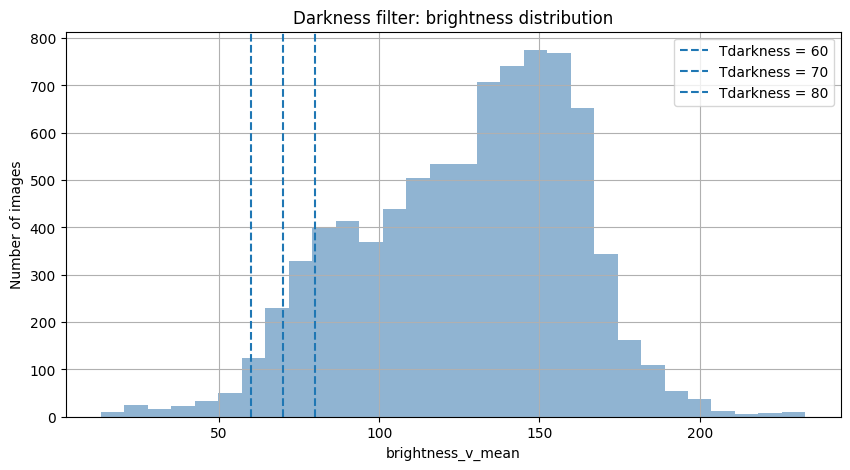
\includegraphics[width=\linewidth]{img/darkness_histogram.png}
  \captionof{figure}{Distribución de la media del canal V para el filtro de oscuridad. Se muestran tres thresholds explorados}
  \label{fig:darkness_hist}
  \end{minipage}
  \end{center}

  \begin{center}
  \begin{minipage}{\linewidth}
  \centering
  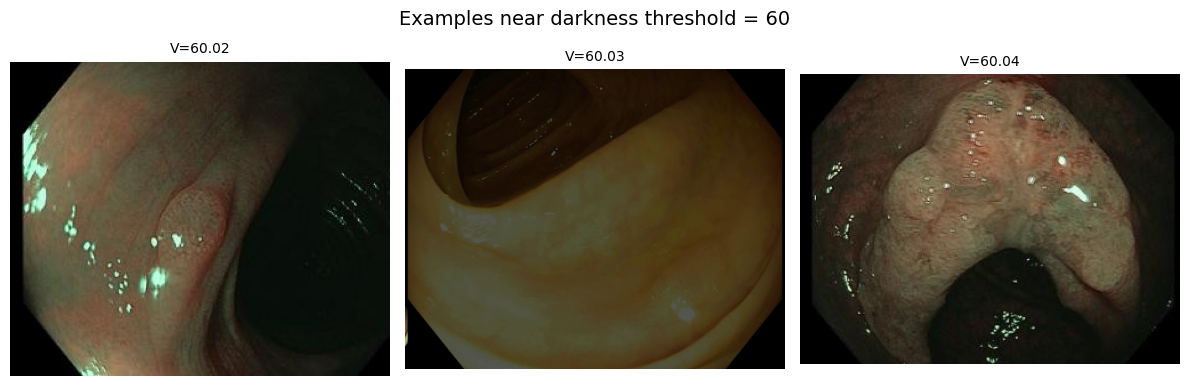
\includegraphics[width=\linewidth]{img/darkness.png}
  \captionof{figure}{Comparación visual de ejemplos cercanos a oscuridad $T=60$.}
  \label{fig:darkness_examples1}
  \end{minipage}
  \end{center}

  \begin{center}
  \begin{minipage}{\linewidth}
  \centering
  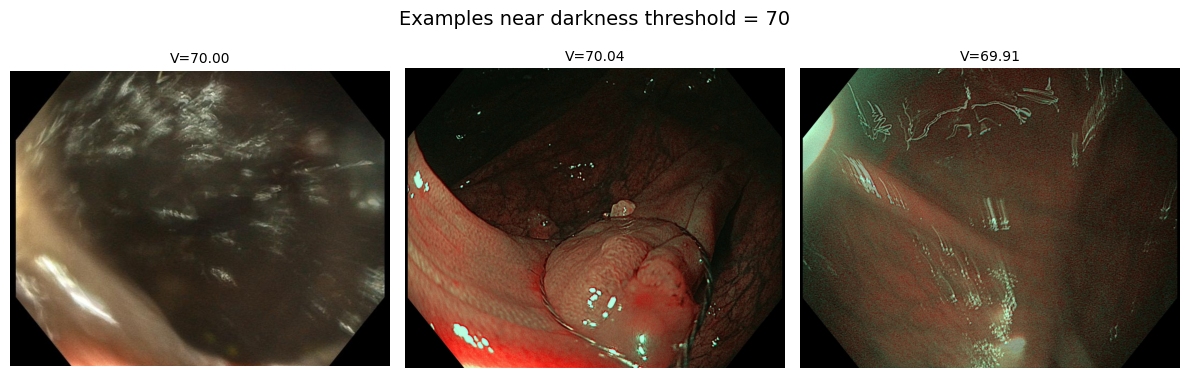
\includegraphics[width=\linewidth]{img/darkness_70.png}
  \captionof{figure}{Comparación visual de ejemplos cercanos a oscuridad $T=70$.}
  \label{fig:darkness_examples2}
  \end{minipage}
  \end{center}

  \begin{center}
  \begin{minipage}{\linewidth}
  \centering
  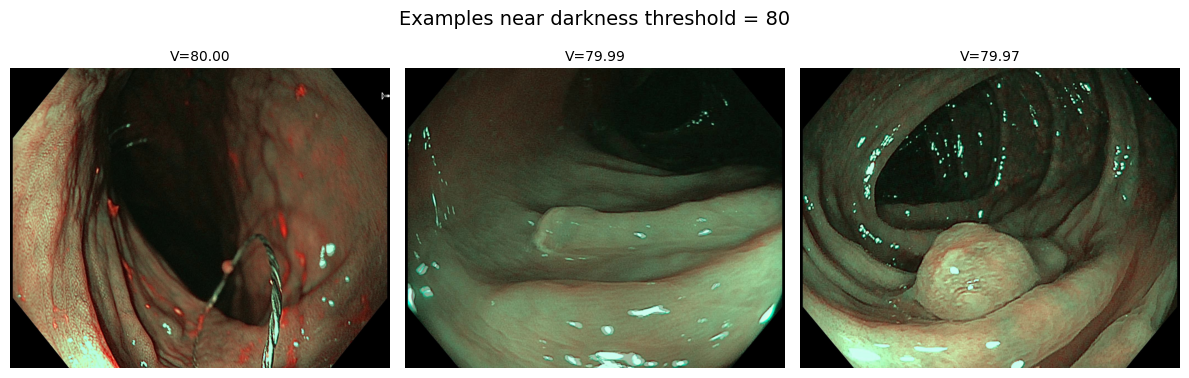
\includegraphics[width=\linewidth]{img/darkness_80.png}
  \captionof{figure}{Comparación visual de ejemplos cercanos a oscuridad $T=80$.}
  \label{fig:darkness_examples3}
  \end{minipage}
  \end{center}

  \item \textbf{Filtro de Lúmen:} Descarta frames de navegación donde gran parte de la imagen muestra una región oscura compatible con el túnel intestinal, dificultando el análisis e indicando que esta parte de la exploración no resulta útil para la detección de un pólipo. A diferencia de un simple umbral por área, este filtro busca identificar regiones oscuras cuya forma y localización sean coherentes con la zona de lúmen. Para ello, se trabaja en escala de grises, restringiendo el análisis al campo de visión central, y se segmentan las zonas oscuras tras un suavizado previo de la imagen. Posteriormente, las regiones detectadas se evalúan según criterios de tamaño, oscuridad, circularidad y separación respecto al borde de la imagen. A partir de estas características se calcula un \textit{lumen score}; si dicho valor es superior al umbral $T_{lumen}=0.06$, la imagen se elimina del dataset.

  La selección de este umbral no se realizó de forma arbitraria, sino a partir de un análisis combinado de la distribución del \textit{lumen score} y de la inspección visual de ejemplos cercanos a distintos puntos de corte. Como se observa en la Figura~\ref{fig:lumen_hist}, se exploraron varios thresholds candidatos alrededor del valor final. A partir de esta distribución y de la comparación cualitativa mostrada en las Figuras~\ref{fig:lumen_examples1}, \ref{fig:lumen_examples2} y \ref{fig:lumen_examples3}.

  \begin{center}
  \begin{minipage}{\linewidth}
  \centering
  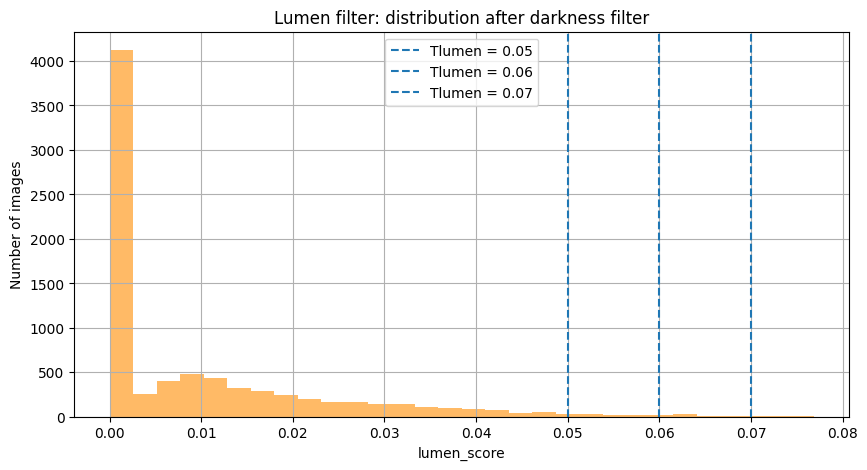
\includegraphics[width=\linewidth]{img/lumen_histogram.png}
  \captionof{figure}{Distribución del \textit{lumen score} para el filtro de lúmen. Se muestran los thresholds explorados.}
  \label{fig:lumen_hist}
  \end{minipage}
  \end{center}

  \begin{center}
  \begin{minipage}{\linewidth}
  \centering
  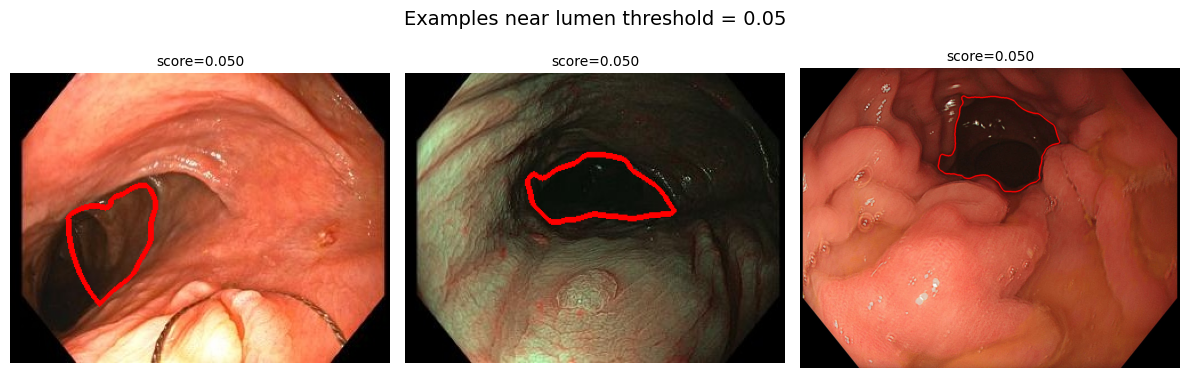
\includegraphics[width=\linewidth]{img/lumen_05.png}
  \captionof{figure}{Comparación visual de ejemplos cercanos a lumen $T=0.05$.}
  \label{fig:lumen_examples1}
  \end{minipage}
  \end{center}

  \begin{center}
  \begin{minipage}{\linewidth}
  \centering
  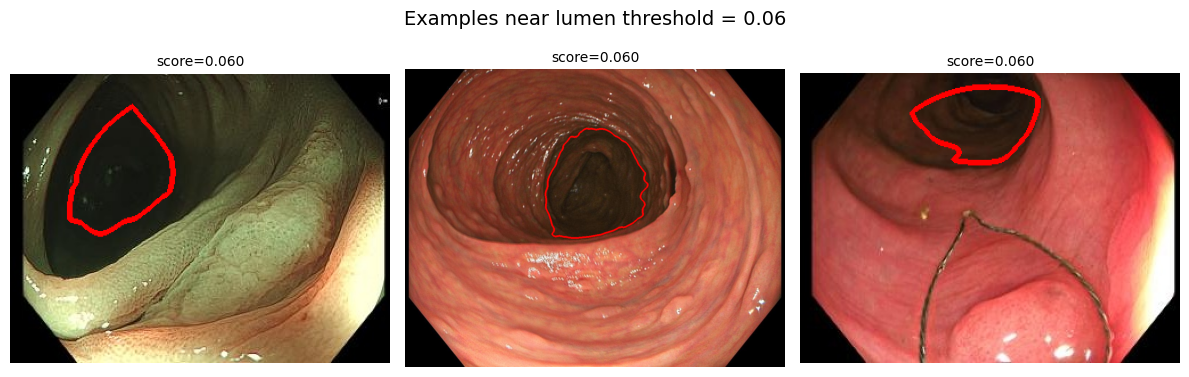
\includegraphics[width=\linewidth]{img/lumen_06.png}
  \captionof{figure}{Comparación visual de ejemplos cercanos a lumen $T=0.06$.}
  \label{fig:lumen_examples2}
  \end{minipage}
  \end{center}

  \begin{center}
  \begin{minipage}{\linewidth}
  \centering
  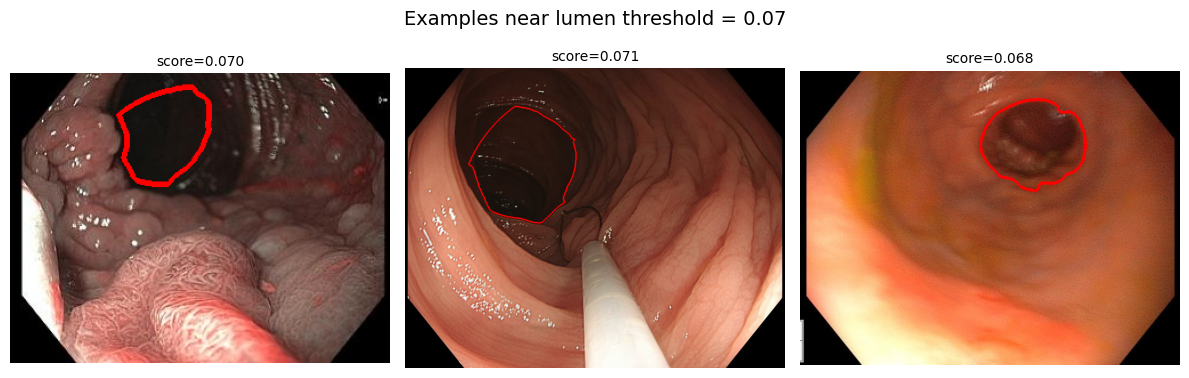
\includegraphics[width=\linewidth]{img/lumen_07.png}
  \captionof{figure}{Comparación visual de ejemplos cercanos a lumen $T=0.07$.}
  \label{fig:lumen_examples3}
  \end{minipage}
  \end{center}

  \item \textbf{Filtro de Uniformidad:} Elimina imágenes donde la cámara choca contra la pared intestinal, generando una imagen de textura plana y borrosa, generalmente roja o rosada. Para detectarlas, se calcula la Entropía de Shannon de cada imagen en escala de grises, utilizándola como medida de la cantidad de información estructural presente en la escena. Si la entropía es inferior al umbral $T_{uniform}=6.3$, el frame se descarta por su falta de textura y detalle visual.

  La selección de este umbral no se realizó de forma arbitraria, sino a partir de un análisis combinado de la distribución de la entropía y de la inspección visual de ejemplos cercanos a distintos puntos de corte. Como se observa en la Figura~\ref{fig:uniform_hist}, se exploraron varios thresholds candidatos alrededor del valor final. A partir de esta distribución y de la comparación cualitativa mostrada en las Figuras~\ref{fig:uniform_examples1}, \ref{fig:uniform_examples2} y \ref{fig:uniform_examples3}, se observó que valores inferiores a 6.0 resultaban demasiado permisivos, ya que seguían conservando imágenes claramente uniformes y sin valor diagnóstico, mientras que valores superiores introducían un descarte demasiado restrictivo al eliminar también frames que todavía contenían cierta estructura útil. Por este motivo, se seleccionó $T_{uniform}=6.3$ como valor de compromiso entre ambas situaciones.

  Con la aplicación de este filtro se han eliminado 152 imágenes, lo que representa apenas un 2\% del total de frames extraídos. Siendo el filtro menos efectivo de los cuatro aplicados, aun así permite eliminar ruido visual de manera clara en un tipo de frame muy específico y perjudicial para el entrenamiento.

  \begin{center}
  \begin{minipage}{\linewidth}
  \centering
  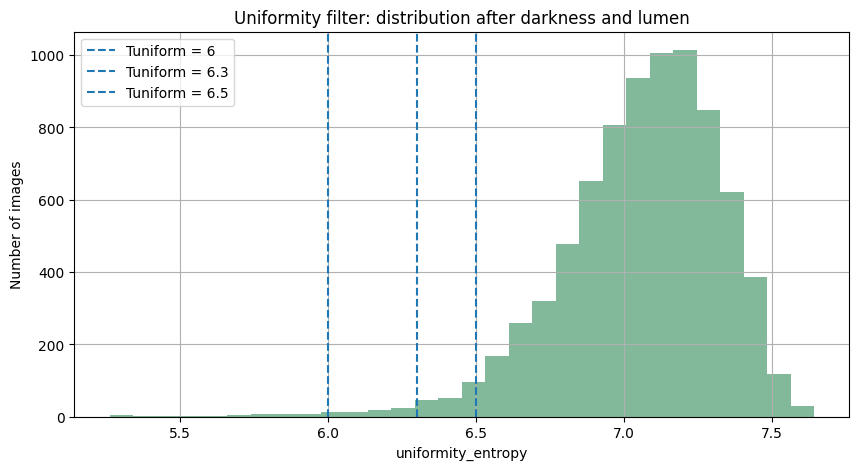
\includegraphics[width=\linewidth]{img/uniform_histogram.png}
  \captionof{figure}{Distribución de la entropía para el filtro de uniformidad.}
  \label{fig:uniform_hist}
  \end{minipage}
  \end{center}

  \begin{center}
  \begin{minipage}{\linewidth}
  \centering
  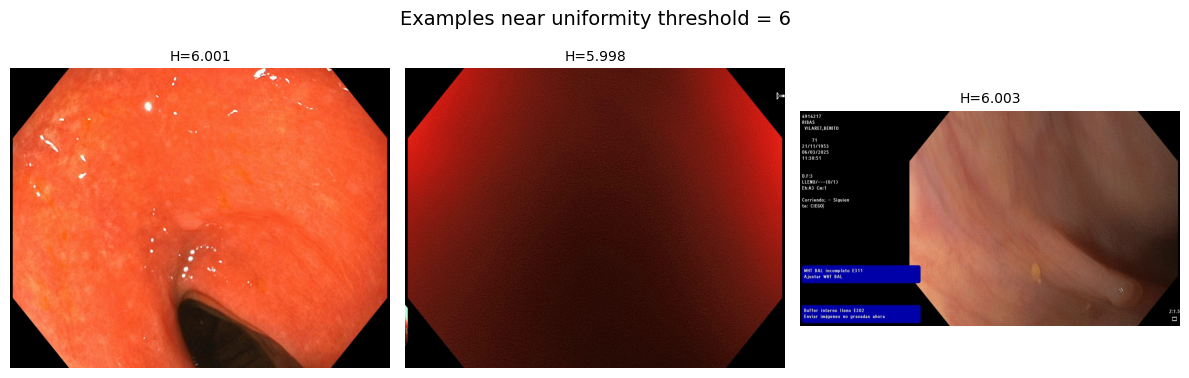
\includegraphics[width=\linewidth]{img/uniform_6.png}
  \captionof{figure}{Ejemplos cercanos a $T=6.0$.}
  \label{fig:uniform_examples1}
  \end{minipage}
  \end{center}

  \begin{center}
  \begin{minipage}{\linewidth}
  \centering
  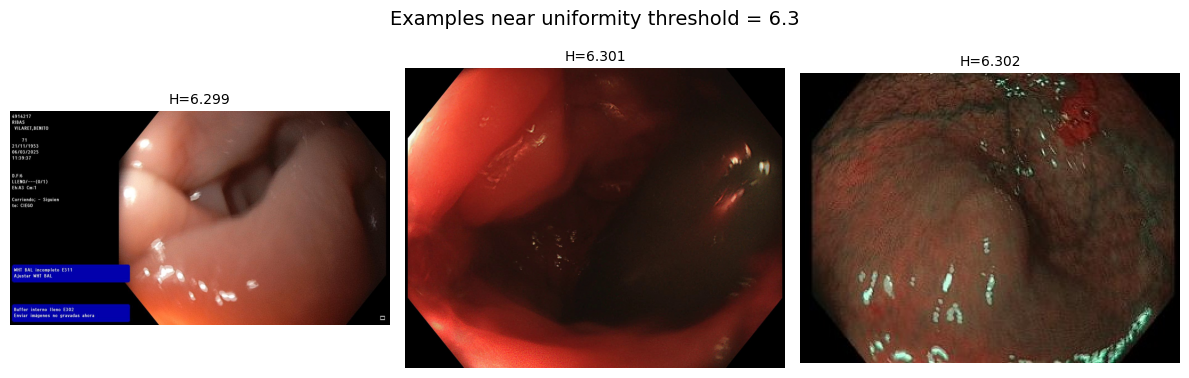
\includegraphics[width=\linewidth]{img/uniform_63.png}
  \captionof{figure}{Ejemplos cercanos a $T=6.3$.}
  \label{fig:uniform_examples2}
  \end{minipage}
  \end{center}

  \begin{center}
  \begin{minipage}{\linewidth}
  \centering
  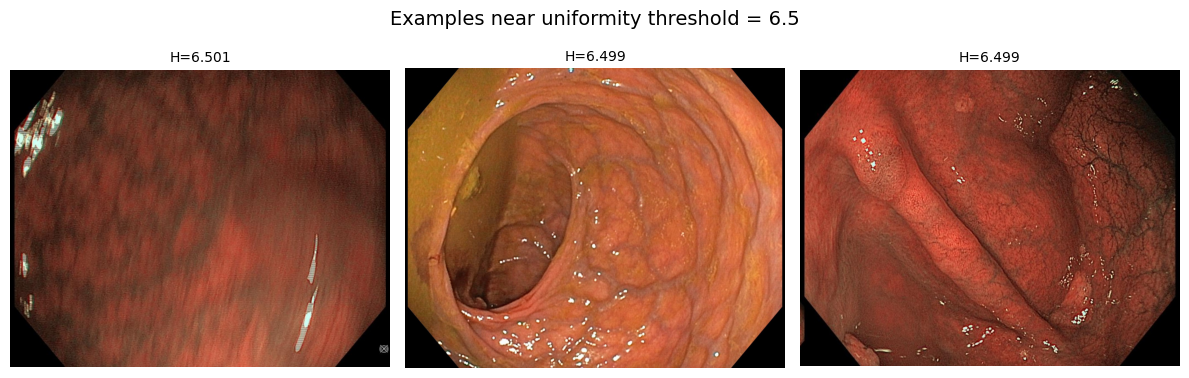
\includegraphics[width=\linewidth]{img/uniform_65.png}
  \captionof{figure}{Ejemplos cercanos a $T=6.5$.}
  \label{fig:uniform_examples3}
  \end{minipage}
  \end{center}

  \item \textbf{Filtro de Desenfoque Extremo:} Detecta la borrosidad causada por el movimiento brusco del endoscopio. Para ello, se aplica un filtro Laplaciano sobre la imagen en escala de grises y se calcula la varianza de su respuesta, utilizándola como medida de nitidez. Las imágenes con una varianza inferior al umbral $T_{lap}=35$ se consideran desenfocadas y se eliminan del dataset.

  La selección de este umbral no se realizó de forma arbitraria, sino a partir de un análisis combinado de la distribución de la varianza del Laplaciano y de la inspección visual de ejemplos cercanos a distintos puntos de corte. Como se observa en la Figura~\ref{fig:blur_hist}, se exploraron varios thresholds candidatos alrededor del valor final. A partir de esta distribución y de la comparación cualitativa mostrada en las Figuras~\ref{fig:blur_examples1}, \ref{fig:blur_examples2} y \ref{fig:blur_examples3}, se observó que valores inferiores a 35 resultaban demasiado permisivos, ya que seguían conservando imágenes con un desenfoque claramente apreciable, mientras que valores superiores introducían un descarte excesivamente restrictivo al eliminar también frames que todavía conservaban suficiente detalle visual. Por este motivo, se seleccionó $T_{lap}=35$ como valor de compromiso entre ambas situaciones.

  Con la aplicación de este filtro se han eliminado 245 imágenes, lo que representa un 3\% del total de frames extraídos, eliminando una cantidad significativa de ruido visual que podría afectar negativamente al entrenamiento del modelo.

  \begin{center}
  \begin{minipage}{\linewidth}
  \centering
  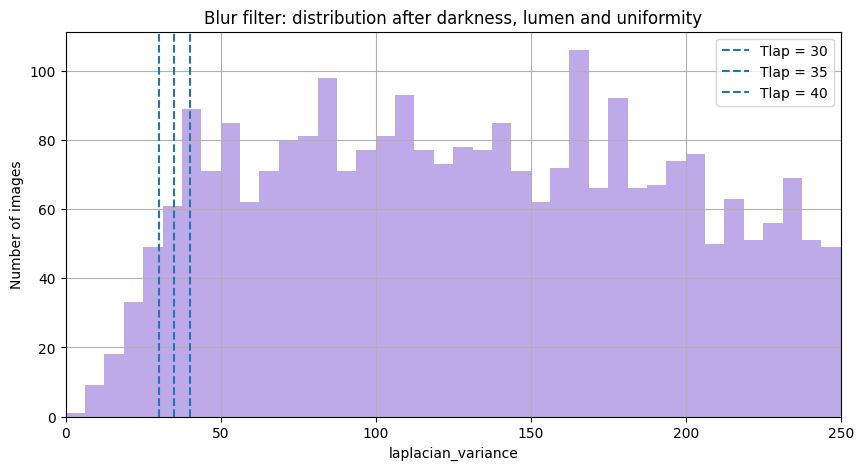
\includegraphics[width=\linewidth]{img/blur_histogram.png}
  \captionof{figure}{Distribución de la varianza del Laplaciano para el filtro de desenfoque.}
  \label{fig:blur_hist}
  \end{minipage}
  \end{center}

  \begin{center}
  \begin{minipage}{\linewidth}
  \centering
  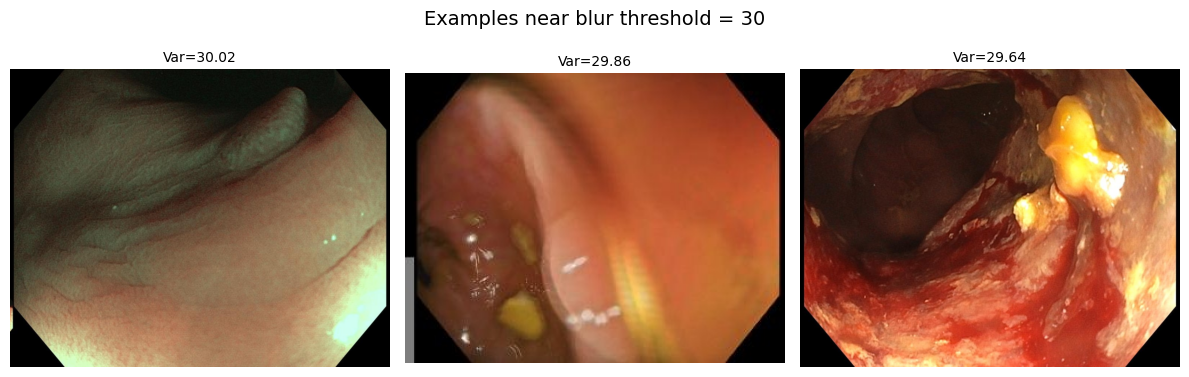
\includegraphics[width=\linewidth]{img/blur_30.png}
  \captionof{figure}{Ejemplos cercanos a $T=30$.}
  \label{fig:blur_examples1}
  \end{minipage}
  \end{center}

  \begin{center}
  \begin{minipage}{\linewidth}
  \centering
  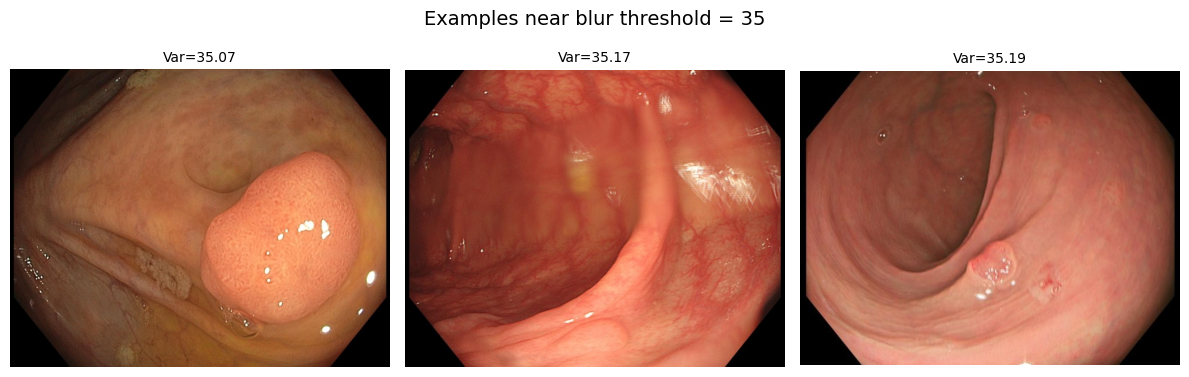
\includegraphics[width=\linewidth]{img/blur_35.png}
  \captionof{figure}{Ejemplos cercanos a $T=35$.}
  \label{fig:blur_examples2}
  \end{minipage}
  \end{center}

  \begin{center}
  \begin{minipage}{\linewidth}
  \centering
  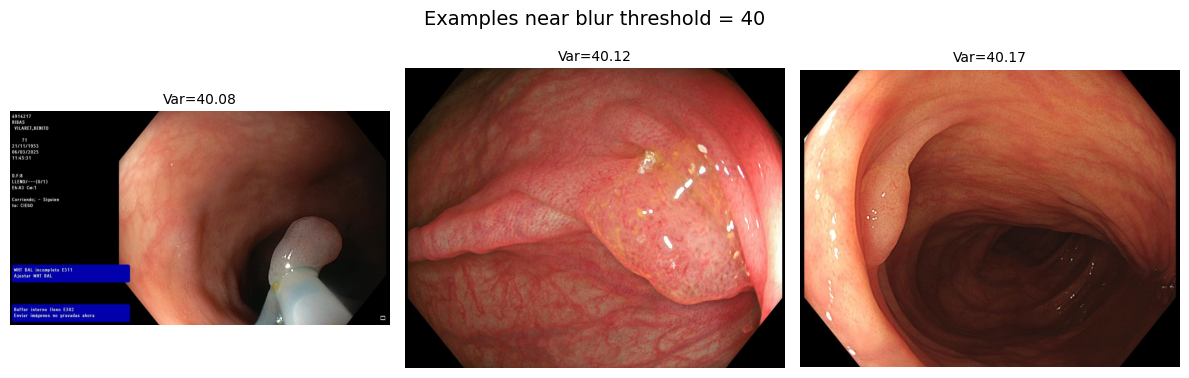
\includegraphics[width=\linewidth]{img/blur_40.png}
  \captionof{figure}{Ejemplos cercanos a $T=40$.}
  \label{fig:blur_examples3}
  \end{minipage}
  \end{center}
\end{itemize}

Tras esta fase 3, el dataset se ha reducido de 8420 a 7692 imagenes, lo que represnenta una reducción de cerca de un 9\% del total de frames extraídos, evidenciando la importancia de esta etapa para mejorar la calidad del dataset. Aún así, esta disminución en el número de imagenes no ha supuesto una mejora tan significativa en el rendimiento del modelo, lo que refuerza la necesidad de seguir con las fases posteriores para conseguir mejores resultados.

\section{Uso de IA}
Durante el desarrollo de este proyecto se han utilizado como apoyo en dos tipos de tareas. En primer lugar, se ha utilizado para la revisión formal del texto, incluyendo aspectos de corrección lingüística y reformulación de párrafos ya redactados. En segundo lugar, se han utilizado como apoyo para comprender conceptos técnicos de visión por computador y deep learning no estudiados previamente.

La herramienta empleada con este fin ha sido Gemini, específicamente el modelo 3.1\cite{google_gemini_2026}

\bibliographystyle{ieeetr}
\bibliography{referencias}

\end{document}
